\subsection{CUDA Fortran}

\begin{frame}[containsverbatim]
	\frametitle{Preliminary remark}

	\begin{itemize}
	\item {lecture based on :\\
		\textbf{CUDA Fortran for Scientists and Engineers}, \\
		Massimiliano Fatica and Gregory Ruetsch, \\
		Morgan Kaufmann, Boston, 2014, \\
		ISBN: 978-0-12-416970-8 \\
	}
	\item {Pre-print available at \url{http://morse.uml.edu/Activities.d/16.520/PS8.D/CUDA_FORTRAN_FOR_ENG.pdf}}
	\end{itemize}
\end{frame}

\begin{frame}[containsverbatim]
	\frametitle{What we'll tackle ?}

	\begin{itemize}
	\item {\textbf{Introduction and basic concepts} what we'll talk about ? }
	\item {\textbf{Memory management} how to best use the different memory levels }
	\item {\textbf{Optimizations} how to better use the Device }
	\item {\textbf{Profiling} \texttt{nvprof} tool and how to find the bottlenecks }
	\item {\textbf{Advanced topics} how to go further ? Multi-GPU, Hybridation with MPI, etc... }
	\item {\textbf{Full example} FDM PDE solver on the Heat Equation }
	\end{itemize}
\end{frame}

\subsubsection{Introduction and basic concepts}


\begin{frame}[containsverbatim]
	\frametitle{Reminder : Terminology}
	\begin{itemize}
	\item {\bf Host :} the CPU and its memory
	\item {\bf Device : } the GPU and its memory
	\end{itemize}
\end{frame}


\begin{frame}[containsverbatim]
	\frametitle{Reminder : Architecture}
	\begin{center}
	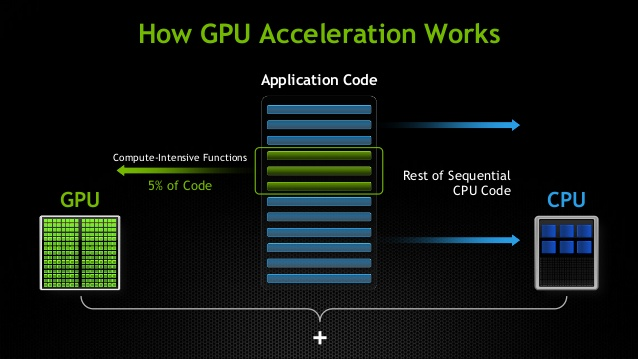
\includegraphics[width=\textwidth]{Day5/images/architecture.jpg}
	\\Copyright : NVidia
	\end{center}
\end{frame}

\begin{frame}[containsverbatim]
	\frametitle{Reminder : Data and instruction offloading}
	\begin{center}
	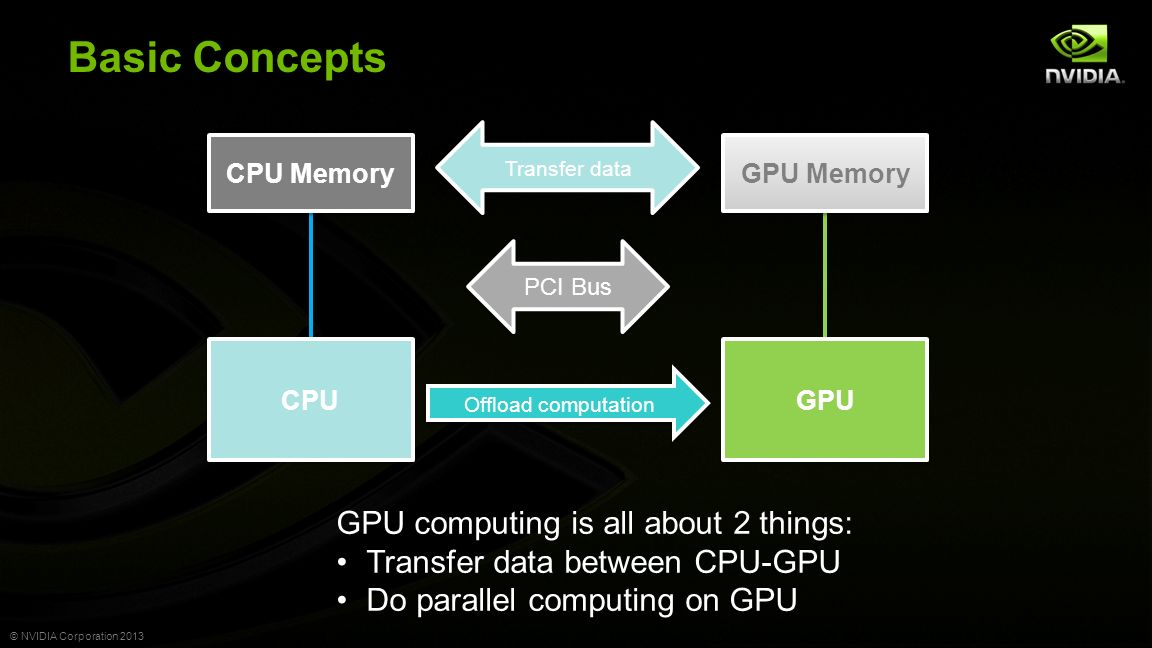
\includegraphics[width=\textwidth]{Day5/images/offloading.jpg}
	\\Copyright : NVidia
	\end{center}
\end{frame}

\begin{frame}[containsverbatim]
	\frametitle{How to compile ?}
	\begin{itemize}
	\item {cross-compiling}
	\item {portland fortran}
	\item {}
	\item {}
	\end{itemize}
\end{frame}


\begin{frame}[containsverbatim]
	\frametitle{Threads hierarchy}
	\begin{itemize}
	\item {A kernel contains one grid "The grid executes on all SMs (Streaming Multiprocessor)"}
	\item {A grid is a grid of blocks "Each block executes on one SM"}
	\item {A block contains threads "The threads in a block are configured to warps"}
	\end{itemize}
\end{frame}

\begin{frame}[containsverbatim]
	\frametitle{Threads configuration}
	\begin{itemize}
	\item {All blocks in a grid are configured the same}
	\item {A specific thread has (1) a bloc-identifier (position in the block) and (2) a grid identifier (position of the block in the grid)}
	\item {}
	\end{itemize}
\end{frame}


\begin{frame}[containsverbatim]
	\frametitle{Kernel launch : the Chevron}

\begin{lstlisting}[language=FORTRAN,frame=lines]
   use my_module
   type(dim3) :: blocksize, gridsize
   
   gridsize = dim3(8,1,1)
   blocksize = dim3(32,1,1)

   call my_function<<<gridsize,blocksize>>>()
\end{lstlisting}
	\begin{itemize}
	\item {First argument : grid configuration}
	\item {Second argument : block configuration}
	\item {In this example : blocksize = 32,2,1 and gridsize = 8,1,1. 512 threads are started on the GPU}
	\end{itemize}
\end{frame}


\begin{frame}[containsverbatim]
	\frametitle{Kernel subroutine attributes}
	\begin{itemize}
	\item {attributes(host) : called/runs on host}
	\item {attributes(global) : called from host, runs on device}
	\item {attributes(device) : called/runs on device}
	\item {attributes(host,device) : generates both versions : host and device}
	\end{itemize}
\end{frame}



\begin{frame}[containsverbatim]
	\frametitle{Kernel}

\begin{lstlisting}[language=FORTRAN,frame=lines]
   module my_module
     use cudafor

   contains

   attributes(global subroutine my_function()
   end subroutine my_function
   end module
\end{lstlisting}
	\begin{itemize}
	\item {}
	\end{itemize}
\end{frame}


\begin{frame}[containsverbatim]
	\frametitle{First example : vector addition}

\begin{lstlisting}[language=FORTRAN,frame=lines]
\end{lstlisting}
	\begin{itemize}
	\item {}
	\end{itemize}
\end{frame}




\begin{frame}[containsverbatim]
	\frametitle{A first CUDA Fortran program}

\begin{lstlisting}[language=FORTRAN,frame=lines]
PROGRAM main
  IMPLICIT NONE
  INCLUDE 'mpif.h'
  INTEGER :: me, nprocs
  INTEGER :: ierr, l=256
  CHARACTER(len=MPI_MAX_PROCESSOR_NAME) :: procname
  CALL MPI_INIT(ierr)
  CALL MPI_COMM_RANK(MPI_COMM_WORLD, me, ierr)
  CALL MPI_COMM_SIZE(MPI_COMM_WORLD, nprocs, ierr)
  CALL MPI_GET_PROCESSOR_NAME(procname, l, ierr)
  WRITE(*,'(a,i2,a,i2,a,a)') 'hello, my rank is', &
      & me,' in a group of', nprocs, ' processes: my name is ', procname(1:l)
  CALL MPI_FINALIZE(ierr)
END PROGRAM main
\end{lstlisting}
\end{frame}


\subsubsection{Memory management}

\begin{frame}[containsverbatim]
	\frametitle{Tiling ...}

	\begin{itemize}
	\item {GPU = multiple SMs}
	\item {To use more than 1 SM, we have to divide the problem}
	\item {Each SM works on one - or more - tile(s)}
	\end{itemize}
\end{frame}

% From : http://geo.mff.cuni.cz/~lh/GUCAS/PDEwPGI2.pdf
\begin{frame}[containsverbatim]
	\frametitle{Different memory levels}
	\begin{itemize}
	\item {Device memory  : using \texttt{DEVICE} attribute}
	\item {Shared memory (on-chip, shared between threads of a block) : using \texttt{SHARED} attribute}
	\item {Constant memory (read-only memory cached on-chip) : using \texttt{CONSTANT} attribute}
	\item {Local Memory : declared as usual on the host}
	\item {Note that the texture memory is not allocatable/usable by the current CUDA Fortran compilers}
	\end{itemize}
\end{frame}




\subsubsection{Optimizations}


\subsubsection{Profiling}


\subsubsection{Advanced topics}

\begin{frame}[containsverbatim]
	\frametitle{C binding}
	\begin{itemize}
	\item {}
	\item {}
	\item {}
	\end{itemize}
\end{frame}



\subsubsection{Full example : FDM solver on the Heat Equation}

% FIXME : http://geo.mff.cuni.cz/~lh/GUCAS/PDEwPGI.pdf








